%%%%%%%%%%%%%%%%%%%%%%%%%%%%%%%%%%%%%%%%%%%%%%%%%%%%%%%%%%%%%%%%%%%%%
%% This is a (brief) model paper using the achemso class
%% The document class accepts keyval options, which should include
%% the target journal and optionally the manuscript type.
%%%%%%%%%%%%%%%%%%%%%%%%%%%%%%%%%%%%%%%%%%%%%%%%%%%%%%%%%%%%%%%%%%%%%
\documentclass[journal=jpcbfk,manuscript=article]{achemso}

%\documentclass[english,aps,preprint,pre,floatfix,nofootinbib,showpacs,showkeys]{revtex4-1}
%%%%%%%%%%%%%%%%%%%%%%%%%%%%%%%%%%%%%%%%%%%%%%%%%%%%%%%%%%%%%%%%%%%%%
%% Place any additional packages needed here.  Only include packages
%% which are essential, to avoid problems later. Do NOT use any
%% packages which require e-TeX (for example etoolbox): the e-TeX
%% extensions are not currently available on the ACS conversion
%% servers.
%%%%%%%%%%%%%%%%%%%%%%%%%%%%%%%%%%%%%%%%%%%%%%%%%%%%%%%%%%%%%%%%%%%%%
\usepackage[version=3]{mhchem} % Formula subscripts using \ce{}

\SectionNumbersOn

\usepackage{amsmath}
\usepackage{amssymb}
\usepackage{color}
\usepackage{CJK}https://www.overleaf.com/project/5e820b28d741e00001b1ccac
\usepackage{framed}
\usepackage[hidelinks]{hyperref}
\usepackage{algorithm}
\usepackage{algpseudocode}
\algdef{SE}[DOWHILE]{Do}{doWhile}{\algorithmicdo}[1]{\algorithmicwhile\ #1}

\usepackage[scaled=0.85]{beramono}
\usepackage[T1]{fontenc}
\usepackage{changepage}

%%%%%%%%%%%%%%%%%%%%%%%%%%%%%%%%%%%%%%%%%%%%%%%%%%%%%%%%%%%%%%%%%%%%%
%% If issues arise when submitting your manuscript, you may want to
%% un-comment the next line.  This provides information on the
%% version of every file you have used.
%%%%%%%%%%%%%%%%%%%%%%%%%%%%%%%%%%%%%%%%%%%%%%%%%%%%%%%%%%%%%%%%%%%%%
%%\listfiles

%%%%%%%%%%%%%%%%%%%%%%%%%%%%%%%%%%%%%%%%%%%%%%%%%%%%%%%%%%%%%%%%%%%%%
%% Place any additional macros here.  Please use \newcommand* where
%% possible, and avoid layout-changing macros (which are not used
%% when typesetting).
%%%%%%%%%%%%%%%%%%%%%%%%%%%%%%%%%%%%%%%%%%%%%%%%%%%%%%%%%%%%%%%%%%%%%

\makeatletter
    \setlength\@fptop{0\p@}
\makeatother

\newcommand*\mycommand[1]{\texttt{\emph{#1}}}

\newcommand{\state}[1]{$\mathcal{S}_{#1}$}

%\newcommand*{\rood}[1]{\textcolor{red}{#1}}
\newcommand*{\rood}[1]{#1}
%\newcommand*{\blauw}[1]{\textcolor{blue}{#1}}
\newcommand*{\blauw}[1]{#1}
%\newcommand*{\groen}[1]{\textcolor{green}{#1}}
\newcommand*{\groen}[1]{#1}
%\newcommand*{\blauwr}[1]{\textcolor{blue}{#1}}
\newcommand*{\blauwr}[1]{#1}

%\newcommand*{\addref}[1]{\textcolor{red}{\{ADD REF: #1\}}}

%\newcommand*{\noter}[1]{\textcolor{red}{[[#1]]}}		% notes on
\newcommand*{\noter}[1]{}					% notes off

%\usepackage[draft]{todonotes}   % notes shown
\usepackage[disable]{todonotes} % notes hidden

%%%%%%%%%%%%%%%%%%%%%%%%%%%%%%%%%%%%%%%%%%%%%%%%%%%%%%%%%%%%%%%%%%%%%
%% Meta-data block
%% ---------------
%% Each author should be given as a separate \author command.
%%
%% Corresponding authors should have an e-mail given after the author
%% name as an \email command. Phone and fax numbers can be given
%% using \phone and \fax, respectively; this information is optional.
%%
%% The affiliation of authors is given after the authors; each
%% \affiliation command applies to all preceding authors not already
%% assigned an affiliation.
%%
%% The affiliation takes an option argument for the short name.  This
%% will typically be something like "University of Somewhere".
%%
%% The \altaffiliation macro should be used for new address, etc.
%% On the other hand, \alsoaffiliation is used on a per author basis
%% when authors are associated with multiple institutions.
%%%%%%%%%%%%%%%%%%%%%%%%%%%%%%%%%%%%%%%%%%%%%%%%%%%%%%%%%%%%%%%%%%%%%
\author{Mike Jones}
\affiliation{%
  Pritzker School of Molecular Engineering, %
  University of Chicago, %
  Chicago, Illinois 60637%
}

\author{Andrew L. Ferguson}
\email{andrewferguson@uchicago.edu}
\affiliation{%
  Pritzker School of Molecular Engineering, %
  University of Chicago, %
  Chicago, Illinois 60637%
}
%\author{I. Ken Groupleader}
%\altaffiliation{A shared footnote}
%\email{i.k.groupleader@unknown.uu}
%\phone{+123 (0)123 4445556}
%\fax{+123 (0)123 4445557}
%\affiliation[Unknown University]
%{Department of Chemistry, Unknown University, Unknown Town}
%\alsoaffiliation[Second University]
%{Department of Chemistry, Second University, Nearby Town}

%\author{Susanne K. Laborator}
%\email{s.k.laborator@bigpharma.co}
%\affiliation[BigPharma]
%{Lead Discovery, BigPharma, Big Town, USA}

%\author{Kay T. Finally}
%\affiliation[Unknown University]
%{Department of Chemistry, Unknown University, Unknown Town}
%\alsoaffiliation[Second University]
%{Department of Chemistry, Second University, Nearby Town}

%%%%%%%%%%%%%%%%%%%%%%%%%%%%%%%%%%%%%%%%%%%%%%%%%%%%%%%%%%%%%%%%%%%%%
%% The document title should be given as usual. Some journals require
%% a running title from the author: this should be supplied as an
%% optional argument to \title.
%%%%%%%%%%%%%%%%%%%%%%%%%%%%%%%%%%%%%%%%%%%%%%%%%%%%%%%%%%%%%%%%%%%%%
\title[]{TBA}


%%%%%%%%%%%%%%%%%%%%%%%%%%%%%%%%%%%%%%%%%%%%%%%%%%%%%%%%%%%%%%%%%%%%%
%% Some journals require a list of abbreviations or keywords to be
%% supplied. These should be set up here, and will be printed after
%% the title and author information, if needed.
%%%%%%%%%%%%%%%%%%%%%%%%%%%%%%%%%%%%%%%%%%%%%%%%%%%%%%%%%%%%%%%%%%%%%
%\abbreviations{IR -- infrared, NMR -- nuclear magnetic resonance, UV -- ultraviolet}
%\keywords{Takens}

\begin{document}
%%%%%%%%%%%%%%%%%%%%%%%%%%%%%%%%%%%%%%%%%%%%%%%%%%%%%%%%%%%%%%%%%%%%%
%% The manuscript does not need to include \maketitle, which is
%% executed automatically.  The document should begin with an
%% abstract, if appropriate.  If one is given and should not be, the
%% contents will be gobbled.
%%%%%%%%%%%%%%%%%%%%%%%%%%%%%%%%%%%%%%%%%%%%%%%%%%%%%%%%%%%%%%%%%%%%%

\newpage

\begin{abstract}

\noindent 

\end{abstract}
https://www.overleaf.com/project/5e9e5110c524b8000192c548
%%%%%%%%%%%%%%%%%%%%%%%%%%%%%%%%%%%%%%%%%%%%%%%%%%%%%%%%%%%%%%%%%%%%%
%% Start the main part of the manuscript here.
%%%%%%%%%%%%%%%%%%%%%%%%%%%%%%%%%%%%%%%%%%%%%%%%%%%%%%%%%%%%%%%%%%%%%

\newpage

\section{\label{sec:intro}Introduction}

Over the last couple decades, DNA has proved to be much more than a vessel for genetic information. From sensing, to computing, to directed self-assembly, the programmable and predictable nature of DNA has unlocked numerous unforeseen applications \citep{Seeman2017DNANanotechnology} (cite more). Recently, structural DNA nanotechnology has enabled self-assembly on micro to milli scales \citep{MhatreV.HoJi-AnnLee2012NIHAccess}, and dynamic DNA nanotechnology has been used to perform basic calculation \citep{Bui2018} and to probe single molecules via temporal DNA signatures \citep{Shah2019}. Both technologies rely on the hybridization reaction between complementary (or similar) DNA strands and leverage the flexibility of shorter DNA oligomers to participate in these reactions. Although many experimental and computational studies have been performed to investigate hybridization and dissociation, the sequence-dependent mechanisms of hybridization dynamics are not fully understood (cite). Moreover, it is unclear whether these processes occur in an "all-or-nothing" fashion or if some metastable states facilitate the transition. The stability of out of register or "slipped" base pairing in repetitive sequences has been well documented in previous computational studies \citep{Phys2014}, \citep{Xiao2019}) and are referred to as slip-strand DNA for longer seqeunces in vivo (cite, maybe too unrelated). Sandstead et al suggested the existence of frayed metastable states during duplex dissociation, where the stability of these states was dictated by oligonucleotide sequence \citep{Sanstead2016}. In this work, we study the same four sequences explored by Sandstead et al in an effort to uncover the sequence-dependent dynamics and their relation to  metastable structures mentioned above.

Given the long timescales on which DNA hybridization and dissociation events occur, the study of these processes are generally not amenable to direct simulation techniques \citep{Phys2014}. Instead, many previous studies of DNA hybridization have employed accelerated sampling methods such as umbrella sampling \citep{Schmitt2013ExploringSurface} transition path sampling \citep{Sambriski2009}, \citep{Hoefert2011MolecularOligonucleotides}  and forward flux sampling  \citep{Phys2014} (cite more). Other studies use dramatically elevated or lowered temperatures to induce one way dissociation and hybridization events, respectively, \citep{Wong2008TheSimulations} (cite more). Experimental studies often employ temperature jump or other perturtabitive methods to drive DNA our of equilibrium and monitor relaxation processes (cite early T-jump and others). Single molecule analysis facilitate equilibrium analysis, however these present technical difficulties and are hampered by long timescales. In this work, we leverage the properties of Markov State Models (MSMs) -- namely that conditional probability depends only on the current state of the system \citep{Pande2010EverythingAsk}--  to run many unbiased coarse-grained simulations and combine these independent simulations to form an understanding of sequence-specific kinetics and thermodynamics. MSMs have recently been implemented to study mechanisms and microstates distribution of DNA hybridization  \citep{Jin2019} \citep{Xiao2019}, but the slowest sequence-dependent kinetics were not the focus of these studies. Pinamonti et al. used MSMs to compare the slowest dynamics of short RNA nucleotides and found that stacking timescales are highly sequence dependent \citep{Pinamonti2017}. We take a similar approach to study 10-mer DNA oligonucleotides and introduce State Reversible Vampnets (SRVs) to directly learn the slowest sequence-dependent dynamical modes \citep{Chen}. Furthermore, we integrate SRVs into the MSM pipeline by generating an optimized low dimensional basis in which microstates clustering can be performed. We show that SRV coordinates can be useful for both directly interpreting dynamical trends and for improving overall MSM quality when compared to more conventional methods such as time-structure independent components analysis (tICA).

Our analysis reflects similar results to previous computational and experimental DNA work, while elucidating some new insights into sequences dependent dynamics and relative timescales. (something here about how this could motivate future experimental work or applications?) By employing SRVs to generate an optimized low dimensional basis, we can access higher resolution MSMs (shorter lag time) and generate a more detailed model. The slow dynamical modes learned by SRVs can be directly compared between sequences to determine otherwise subtle trends. More summarizing results here ..... 


\section{\label{sec:methods}Methods}

\subsection{\label{sec:methods}3spn2 Model}
Not sure if this is necessary, but can include a quick summary of model, why we chose to use it, and interesting features.
-Compatible with lammps
-Enough resolution to deserve dynamical behavior, coarse enough to run equlibrium sims
-Previous hybridization experiments show good agreement with experiments

\subsection{\label{sec:methods}Simulation set up}

We initialized four sequences previously investigated by Sandstead et al \citep{Sanstead2016} -- AT-all, GC-core, GC-end, and GC-mix -- (small figure here) along with their complementary strands according a Beta helices according to 3SPN.2 documentation \citep{Phys2014}. We initialized explicit ions such that 240 mM NaCl and 18 mM MgCl2 were added to the box in addition to 18 Na counter ions to balance the charge from the 9 phosphate groups in each oligonucleotide backbone \citep{Hinckley2015}. In order to maximize concentration without allowing strands to see each other through periodic boundaries, we set the box size just larger than the sum of the maximum end to end extension length of a single strand and the force cutoff (using Ewald summation method is set at 20 A). This translated to a box size of 77.74 A and an effective oligo concentration of 7 mM. We used an Ewald potential to calculate long range Coulombic interaction between DNA and ions. We maintained a Debye-Huckel screening potential with an ionic strength of 240 mM -- corresponding to NaCl concentration -- to account for phosphate backbone interactions. These electrostatics preserve the persistence length and intrinsic curvature of DNA while taking the effects of ion-DNA interactions\citep{Hinckley2015}. We run our simulations in the NVE ensemble and fix temperature via a Langevin thermostat in order to model implicit solvent interactions \citep{Schneider1978Molecular-dynamicsTransitions}. Simulation temperature was determined by sequence specific melting temperature such that strands were about equally likely to spend time in the hybridized or dissociated state. Tmelt simulations were run for $3*10^{8}$ time steps, equating to 4.5$\mu$s simulation time, and frames were saved every 30 ps. A 15 fs timestep was used for all simulations runs. For each sequences, 100 simulations were performed in parallel, consuming about 32 serial cpu-hours of computation time for each independent simulation. An approximate Tmelt Boltzman distribution was replicated by initializing half of runs from the hybridized state and half from a random dissociated state. In order to allow for further equilibration, the first third (1.5 $\mu$s) of each simulation was removed, resulting in 100 x 100000 frames and a total of 300$\mu$s simulation time per sequence.

\subsection{\label{sec:methods}Featurization}

All intermolecular pairwise distances for both oligonucleotides were calculated at each frame using MDtraj software package \citep{McGibbon2015MDTraj:Trajectories}. Based on the self-complementary nature of each sequence, we averaged permutable distances (45 pairs in total) together. This permutation reduction follows a similar procedure used in TICAgg coordinates construction \citep{Sengupta2019AutomatedSelf-assembly}. The VAMP-2 scoring method, which represents the sum of squared estimates for the transfer operator, was employed to evaluate the quality of this feature set \citep{Mardt2018VAMPnetsKinetics}. We compared the VAMP-2 score (SI ?) for the permutation-free distances to the complete set of intermolecular distances and found only a small loss in kinetic variance when using the reduced data set. Furthermore, we found an increase in VAMP-2 score when using reciprocal pairwise distances and chose these reciprocal permutation-free coordinates as a consistent feature set. These features were normalized and passed into sequence-specific SRVs. 

\subsubsection{\label{sec:methods}SRVs}

SRVs were first developed by Chen et al. as a means to directly learn slow eigenfunctions of the transfer operator \citep{Chen}. The framework uses a twin-lobed artificial neural network, similar in structure to the network employed in VAMPnets \citep{Mardt2018VAMPnetsKinetics}, to learn a low dimensional representation of input features. This representation is optimized for the variational approach to conformational dynamics (VAC) from which the leading eigenfunctions of the transfer operator can be estimated (equation here?). The resulting orthogonal modes are associated with the slowest dynamical processes in a system, and can be used to interpret kinetic information directly (such as physical correlations and timescales) and to construct markov state models. Other methods, such as time-lagged independent component analysis (TICA) and kernel TICA (kTICA), have been employed in place of SRVs but suffer limitations from the linear transformation in the case of the former and high computational cost in the case of the latter \citep{Harrigan2017LandmarkDynamics}. SRVs provide robust nonlinear approximation and computation timescales linearly with the amount of input data. This is a key attribute to our system as 10 million frames with 55 features in each frame are used as input data. The SRV framework has been tested on toy systems where the true eigenfunctions of the transfer operator are known and on small protein simulation data such as the WW-domain and Trp-cage mini-protein (cite). For these latter system, SRV-MSMs were contructed in order to find the stability of metastables states as well as transition probabilities between those states.

Using optimized hyperparameters and featurized trajectory data, we generated a hierarchical dynamic encoder (HDE) to transform 55 reciprocal pairwise distances into a low dimensional SRV feature set. In order to maintain consistency between sequences, we kept all SRV training hyperparameters the same with the exception of the number of outputed slow modes. We determined the number of slow mode via cross-validation on the VAMP-2 score to ensure that the coordinate did not over fit on statistical noise \citep{McGibbon2015VariationalKinetics}. In particular we looked for a diminishing increase in the vamp-2 score, inconsistency between cross validation scores -- suggesting that the model maybe learning different modes, and a widening gap between train and test scores -- suggesting that the model might be overfitting on statistical noise in the training data. We used a batch size of 50000 and ran each model for total of 30 training epochs. We used two hidden layers and set the size of each layer to 100. For cross-validation and comparison between different hyper-parameters, we used a 80/20 validation split training. SRV training required about 22 GPU-minutes across 1 GPU and 10 CPUs.

\begin{figure}[ht!]
	\begin{center}
        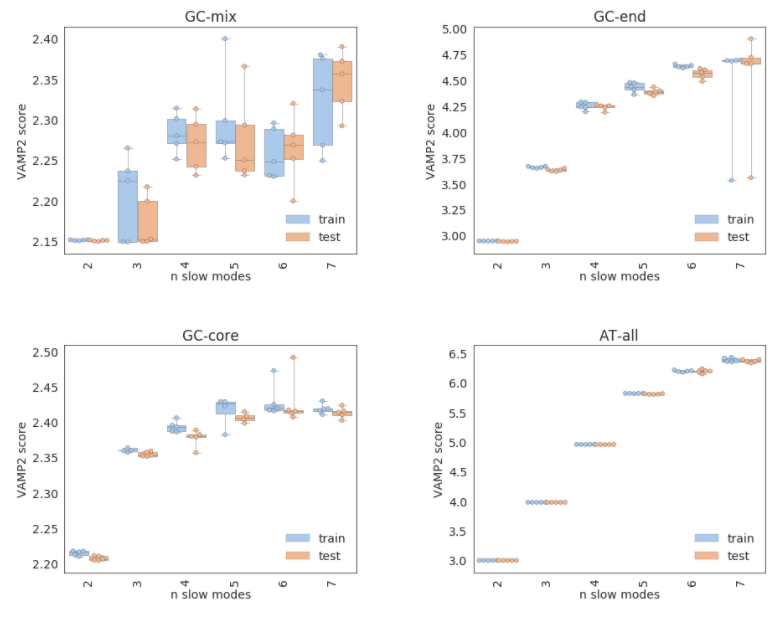
\includegraphics[width=\textwidth]{Figs/figs_0804/srv_crossval.png}
        \caption{Cross val procedure to selection number of SRV coordinates (probably will be SI, but could include AT-all cross-val in the walkthrough section)}
        \label{fig:srv_crossval}
	\end{center}
\end{figure}

\subsubsection{\label{sec:methods}SRV-MSMs}

MSMs are a powerful tool for interpreting large amounts of simulation data in a statistically robust and experimentally comparable way. The technique relies on the discretitization of kinetically similar conformations into microstates and finds the conditional probability between states within some lag time. The reliance on conditional probabilities allows for many independent simulations (longer than the lag time) to be collectively interpreted. To take full advantage of the MSM frameworks, however, the input basis should be as kinetically meaningful as possible \citep{Pande2010EverythingAsk}. This becomes crucial in our system given the large difference in timescales between leading modes. Because SRV eigenfunctions translate simulation features into their slowest kinetic representations, they are optimally suited as an MSM basis. To prove this, SRV-MSM VAMP-2 scores were shown to be consistently higher than MSMs constructed from TICA coorinates (TICA-MSMs) \citep{Sidky}. Furthermore, SRV-MSM implied timescales converge faster than TICA-MSM timescales, enabling a shorter lag time and therefore a higher resolution model. To build our SRV-MSM framework, we employed the Pyemma MSM pipeline and generated independent models for each sequence \citep{Scherer2015PyEMMAModels}. After passing in SRV coordinates, we perform k-means microstate clustering, Bayesian MSM construction, and PCCA+ macrostate assignments. The number of microstates were determined by VAMP-2 score, and the SRV-MSM lag time was selected based on implied timescales convergence.  The number of PCCA+ macrostates was determined based on the characteristic of each system and will be discussed more in depth in the results. 


%%%%%%%%%%%%%%%%%%%%%%%%%%%%%%%%%%%%%%%%%%%%%%%%%%%%%%%%%%%%%%%%

\section{\label{sec:Results}Results}
- lead with same kind of diagram for each sequence, add additional figures when necessary for a given sequence

\subsection{\label{sec:Results}AT-all}
\subsubsection{\label{sec:Results}Explanation of state selection and slow modes}

In our analysis, we found that the AT-all sequence, given its repetitive structure and lack of GC-content, produced the cleanest dynamics and displayed a canonical spectral gap between modes. For this reason, we lead our discussion with this sequence and use it as a case study to work through our SRV-MSM pipeline step by step. Our first task was to identify the SRV lag time that was longer than the intrinsic Markov timescales of the system, yet short enough to resolve the dynamics of interest \citep{Phys2018MarkovValidation}. We found that most implied timescales (with the exception of the leading timescale) converge at a lag time of 600 ns. We kept a looser constraint on the convergence of the leading mode as it reflects the less Markovian dynamic of strand association and dissociation (*not sure if this warrants further discussion). It should be noted that our lag time selection was informed by the other sequences as well to maintain consistency. Next we selected an optimal number of SRV components to include in our analysis. After a certain point, higher order dynamical modes provide diminishing contributions the overall kinetic variance as measured by the Vamp-2 score, and the model can begin fitting on statistical noise in the trajectory data instead of the true dynamics \citep{McGibbon2015VariationalKinetics}. It is also more difficult to perform kmeans clustering on a high dimensional space, especially when those higher dimensions are less kinetically relevant \citep{Pande2010EverythingAsk}. For these reasons, the number of slow SRV components should be carefully selected based on the specific system of interest. For the AT-all sequence, we generate SRVs with five components, representing the five slowest processes in the systems. Next, we seek to interpret the physical relevance of these leading modes by plotting the Pearson correlation of each mode with the 100 intermolecular distances between strands. The quantitative meaning of these coordinates can be difficult to interpret given their nonlinear relationship to the SRV collective variables, but the relative different between these correlations shows which coordinates are most affected by each process. For example, the first slow mode shows a significant positive correlation to each distance and the strongest correlation with matching base pair distances (shown along the main diagonal). Given these relationships and the substantially longer timescale of this process, we can deduce that this leading mode corresponds to the dynamics of the overall hybridization and dissociation process. The next four SRV components all show a relatively high correlation along different offset diagonals. These diagonals correspond to the intermolecular distances between shifted base pairs (SI figure for this?), and point to the existence of gradually faster sliding or "slithering" processes. Slow slithering mechanisms have similarly been reported in simulation studies to occur on orders of magnitude longer timescales than some  underlying fast dynamics \citep{Markegard2015}, \citep{Xiao2019}. 

\begin{figure}[ht!]
	\begin{center}
        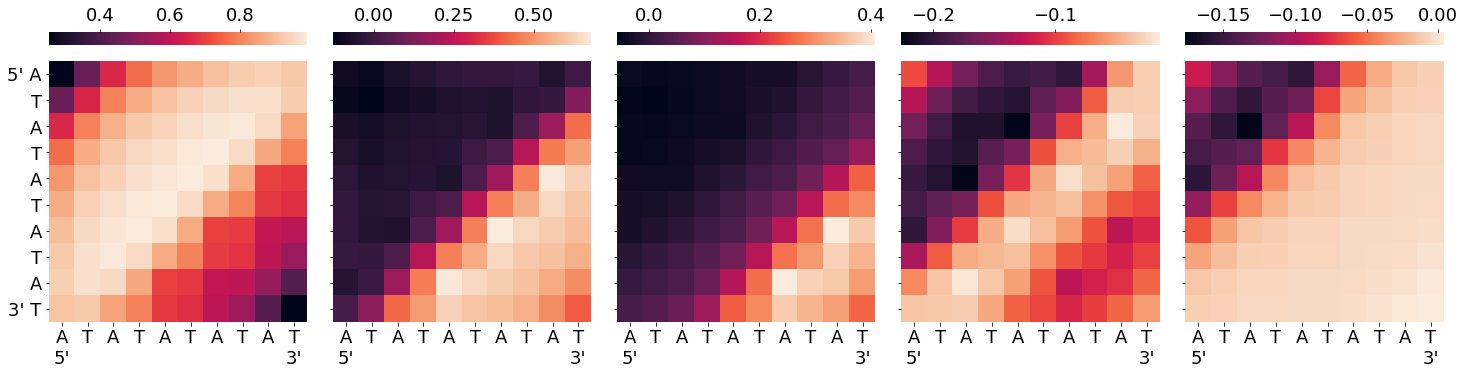
\includegraphics[width=\textwidth]{Figs/figs_0804/AT-all_srv_correlations.png}
        \caption{Shows Pearson correlations between leading SRV modes and all 100 intermolecular distances (needs labels for slow modes)}
        \label{fig:AT-all_srv_correlations}
	\end{center}
\end{figure}

From this analysis we can determine that the slowest dynamics are fully characterized by the hybridization process and slithering behavior of out of register base pairs. Although this is qualitatively informative, we can access a more holistic picture of sequence kinetics and thermodynamics by using these SRV coordinates as a basis on which to construct an MSM. Because these coordinates are already capturing a majority of the system's kinetic variance, they serve as an ideal basis on which to group frames into microstates. We performed k-means clustering, and optimized the number of microstates at 200 by monitoring VAMP-2 score. Next, we selected an MSM lag time in a similar fashion to our SRV lag time selection process. In the figure (dynamical figure) we compare the convergence of SRV-MSM and TICA-MSM timescales, where SRV-MSM timescales converge consistently faster and to higher values of all leading modes. This enables us to select a shorter lag time and build a higher resolution model than we could from an analogous TICA basis. Using an MSM lag time of 1.2 ns, we then built a Bayesian MSM to calculate transition probability matrix between each microstate. Finally, PCCA+ spectral clustering was implemented to group these microstates into macrostates that each represent a collection of metastable structures. Previous work have used a common set of microstates and/or performed manual clustering of microstates based on physical read outs from simulation data (stacking score, energies, etc) \citep{Pinamonti2017PredictingModels}, \citep{PinamontiAnalyzedModels}. Although these techniques are useful for performing comparisons between sequences, we saw better results when optimizing MSMs to capture the most detail of sequence individually and thus developed an independent set of microstates and macrostates for each sequence. For AT-all, we kept to the convention of clustering into n+1 macrostates, where n is the number of slow components captured by the MSMs. To visualize these six macrostates, we project the data into the two leading TICA coordinates. Although SRVs outperform these coordinates for the purpose of MSM construction, TICA represent good high variance collective variables on which to visualize free energies and state assignments \citep{Sidky}. It is clear in figures (thermo fig) that the PCCA state assignments are capturing free energy minima in TICA space as independent states. After assigning these macrostates we can then calculate their relative probabilities and free energies, visualize representative molecular renderings, and estimates transition probabilities between states. In this final step, we use a minimum flux cutoff of 2e-6 in order to mitigate erroneous quick transition or skipping between states. 

\begin{figure}[ht!]
	\begin{center}
        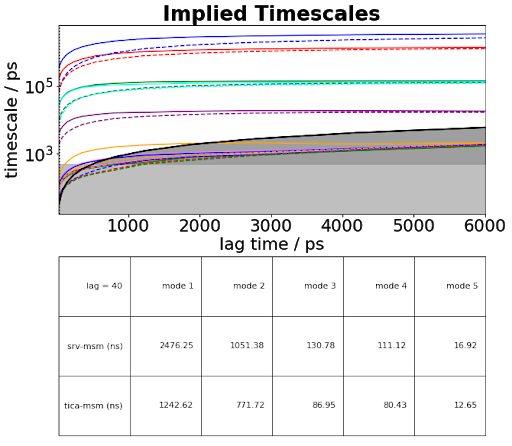
\includegraphics[width=\textwidth]{Figs/figs_0804/AT-all_dynamic.png}
        \caption{SRV-MSM timescales convergence and implied timescales using a lag time of 1.2 ns}
        \label{fig:AT-all_dynamic}
	\end{center}
\end{figure}

In our coarse-grained SRV-MSM, we observe an "aligned hybridized" state, dissociated state, and four "shifted" states characterized by different combinations of out-of-register base pairings. These shifted states consist of 2 or 4 base pair shifting (single or doubled shifted) in either the 5' or 3' direction with varied stability and transition fluxes between kinetically neighboring states. This state decomposition is expected given the repetitive nature of the AT-all sequence and previous computational results that find shifted conformations form "deep kinetic traps" \citep{Xiao2019}, \citep{Phys2014}. We found a substantial difference in thermodynamic stability and kinetic behavior between the 5'A shifted states and 3'T shifted states. This difference can be accounted for by examining experimental studies on the thermodynamics of "dangling ends" -- unpaired bases adjacent to the paired duplex -- and "inert tails" -- free bases that extend beyond the dangling end \citep{Michele2014EHybridization}. Dangling 5' ends have a consistently stabilizing effect, and inert tails decrease stability as they increase in length. It has been shown that two base pair 5' dangling ends (or say one base pair inert tails) have higher melting temperature and are enthalpically favorable compared to 3' ends \citep{Senior1988InfluenceDuplexes}, \citep{Dickman2012ThermodynamicDNAs}. This is likely due to 5' ends preferentially stacking on the core duplex compared to 3' ends. Furthermore, Santalucia thermodynamic calculations reveal that the specific nearest neighbors bonds in the 5' shifted state are more energetically favorable than those in the 3' shifted state \citep{Allawi1998NearestDNA} (NN calculations SI?). Taken together, these experimental results substantiate why we observe the single shifted 5' state to be only slightly less stable relative to the aligned hybridized state. Moreover, it is expected that implied timescales corresponding to this process is on the same order of magnitude at the hybridization timescale. The stability of the single shifted 3' state is notably lower and on the same order of magnitude as the double shifted 5' state despite it having two less intact base pairs. The final state is more stable than one might expect given the difference in stability between the single and double 5' shifted states. Experimental work  \citep{Doktycz1990ThermodynamicATGC} studied four base pair dangling ends on DNA hairpins, and found that TATA ends are most stabilizing than ATAT. Although NN interactions paly a more important role in determining stabiity, this could explain why the relative free energy difference between single shifted 3' state and double shifted 3' is not as large as the difference between the single shifted 5' and double shifted 5' states.

\begin{figure}[ht!]
	\begin{center}
        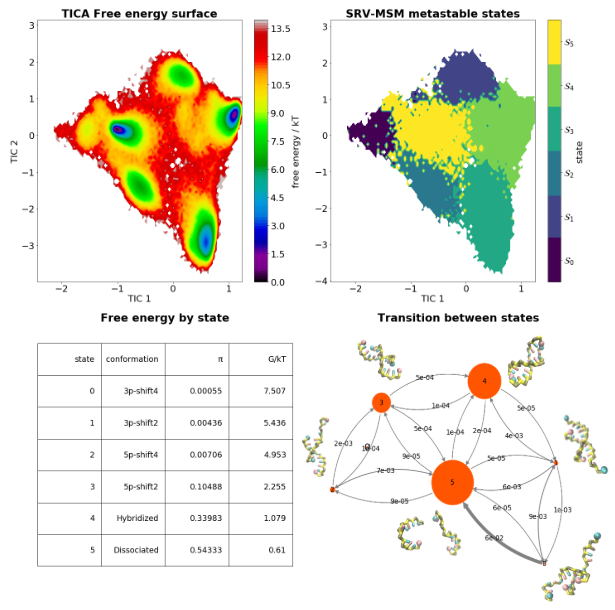
\includegraphics[width=\textwidth]{Figs/figs_0804/AT-all_thermo.png}
        \caption{SRV-MSM TICA projection, state free energies, and transitions probabilities}
        \label{fig:AT-all_thermo}
	\end{center}
\end{figure}

Beyond state probabilities and free energy approximations, the macrostate MSM also yields discrete kinetic information in the form of transition probabilities between states. Figure (thermo fig) show the probability of moving from one state to another within the MSM lag time (1.2 ns). All transition probabilities are higher when moving towards a more aligned state than towards a more shifted state, suggesting that these metastable shifted states play a more significant role in facilitating the hybridization process than dissociation. Furthermore, we see equal or higher transition rates from shifted states to the dissociated state than to more aligned states, indicating that the slithering-hybridization process is readily disrupted by complete dissociation. In particular, we observe that the transition probability from double shifted 3' state to the dissociated state is 6x higher than to the neighboring single shifted 3' state. From this we conclude that shifted states are important in facilitating the hybridization process, but that a higher degree of shiftedness (in particular when shifted in the 3' direction) is less likely to evolve into a fully aligned hybridized state than it is to dissociate in the process.

For all proceeding sequences, we use the same SRV and MSM lag times, number of microstates, and cross-validation procedures as in the AT-all case. Although these might not represent fully optimized hyperparameters for each sequence, they preserve Markovian properties of the system and provide adequate resolution to evaluate macrostates. The number of SRV coordinates and MSM macrostates are varied based on the kinetics and thermodynamics behavior of specific sequences.

%%%%%%%%%%%%%%%%%%%%%%%%%%%%%%%%%%%%%%%%%%%%%%%%%%%%%%%%%%%%%%%%

\subsection{\label{sec:Results}GC-end}
	
Next we examine the GC-end sequence, which add GC caps to the same repetitive AT motifs. Based on SRV cross-validation (SI) we use the leading four slow modes to define our MSM basis.  These coordinates are qualitatively similar to those we studied for AT-all, where the three faster modes each represent some slithering dynamics. When we build the SRV-MSM for the GC-end sequence we observe a larger separation between the leading SRV-MSM timescale and the proceeding modes, which is shown in figure (SI fig) by a distinct spectral gap. We observe a second spectral gap after the fourth slow modes along with a drop in the model vamp-2 score. The clustered macrostates show a similar distribution where shifted populations are notably lower. The 3' double shifted state is no longer identified as a metastable state, and the total number of states is reduced to five (again one more than the total number of slow modes). Although these states appear similar to the AT-all shifted states, the presence of the C:T or G:A mismatches decreases the number of out-of-register WC pairs by two relative to corresponding AT-all states. This substantially diminishes the stability of the GC-end shifted states, resulting in lower state populations and lifetimes.

\begin{figure}[ht!]
	\begin{center}
        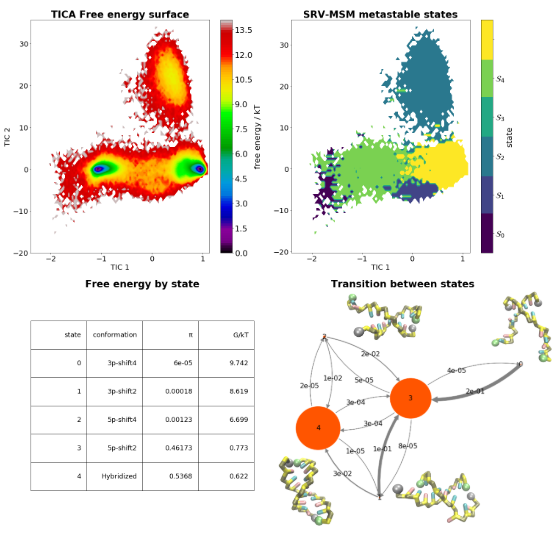
\includegraphics[width=\textwidth]{Figs/figs_0804/GC-end_thermo.PNG}
        \caption{Shows Pearson correlations between three leading SRV mode and all 100 intermolecular distances (not sure why there are 6 color on the legend since there are only 5 states, need to fix this)}
        \label{fig:shifting_distributions}
	\end{center}
\end{figure}

For our analysis, we consider C:T and G:A base pairs in the GC-ends shifted states as non-interacting dangling ends. Although such internal mismatches of this kind may cause substantial conformational distortions such as kinking, terminal mismatches have been shown to be slightly stabilizing \citep{Santalucia2004TM}, \citep{DiMichele2014EffectHybridization}. In the context of the 3spn2 model, these ends are accounted for via intra-strand base stacking and inter-strand cross-stacking interactions \citep{Hinckley2013AnHybridization}. The only interaction between non-WC basepairs is parameterized by isotropic excluded volume potential, which is likely much more simplistic than the true mismatch bond and can therefore not represent the state with highest fidelity. Nevertheless, we find these bonds to be stabilizing enough to account for the relatively small population of conformation we observed in these shifted states (NN calculations). Interestingly, we found that 5' single shifted stability might be elevated by a substantial portion of conformations retaing one intact GC base pair. Visualizations reveal that the shifted oligos -- particularly in the 5' shifted state -- have a tendency to sacrifice some helical conformational entropy in a way that facilitates an out of register GC base pairs. To compare these single shifted 5' prime states with the corresponding AT-all state, we employ diffusion maps built on an equal sampling of 10000 conformations in both states. Diffusion maps generate a low dimensional embedding based on some metric for diffusive distance (we use intermolecular distances) and are well-suited to find subtle structural differences in temporally disconnected data \citep{Coifman2006DiffusionMaps}. The first diffusion mode clearly delineates between the GC-end and AT-all shifted conformations and correlates highly with the average distance between the 3' end and its shifted complementary pair. This reveals that the mismatch GC-pairs are never bound -- a consequence of the excluded volume interaction -- whereas the AT-all pairs are mostly bound with occasional fraying indicated by small AT-all overlap in the GC-end region. On y-axis we examine the second diffusion mode, which correlates highly with the average distance between 3' and 5' ends. Because the GC-end termini do not bind out of register, we find that they are readily able to form stabilizing contacts despite the shifted conformation of the duplex as a whole. These "shifted-loop" bonds are shown to be uniquely stable for GC-end conformations, and their existence in the simulations confirmed by molecular renderings of these regions. 

It is unclear the extent to which these interactions are physical given the strain required to form these shifted loops (need to discuss toehold loop experiments with Brennan).  Single shifted 3' and double shifted 5' strands have much lower population of these shifted loops (need to perform calculations to see if these account for increased stabilization of single shifted 5' versus single shifted 3'). Not sure how much more much to go into here ...

\begin{figure}[ht!]
	\begin{center}
        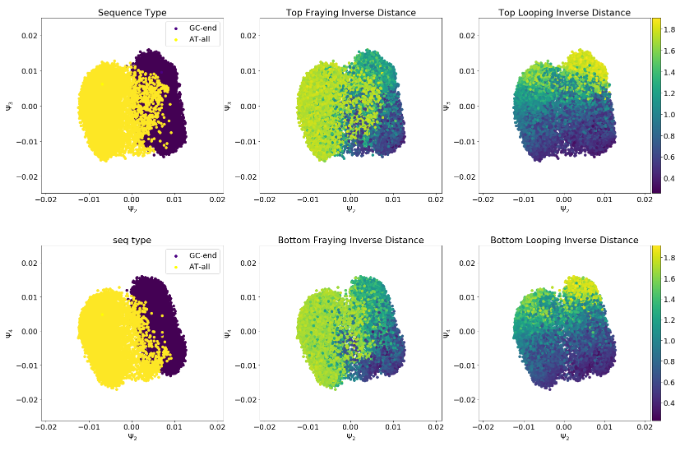
\includegraphics[width=\textwidth]{Figs/figs_0804/diff_maps_full.png}
        \caption{First three diffusion map coordinates built from 20000 single shifted 5' states, equally sampled from AT-all and GC-end. (need to add some molecular rendering of states).}
        \label{fig:shifting_distributions}
	\end{center}
\end{figure}

The dynamic picture looks fairly different for the GC-end macrostates compared to AT-all. We do not observe any significant flux between the double shifted to single shifted 5' states. While this could be due to insufficient sampling, it is likely that the double shifted states has too few contacts to directly transition into a single shifted state without first dissociating. This is further demonstated by the kinetic distance between this state and the aligned hybridized state (S0 and S4, respectively) shown in TICA projections (thermo figure).We observe some flux between the single shifted states and aligned hybridized state, but these events are more rare than their AT-all equivalents. This suggests that although these transitions are possible routes for hybridization/dissociation, it is substantially more common for the transition to proceed in a two-state manner. In T-jump experiments, the GC-end sequences was observed to have less deviation from the two-state dissociation model compared to oligonucleotides with GC pairs closer to the core \citep{Sanstead2016}. Further analysis showed a unknown kinetic response was recorded for GC-end sequence -- particularly at lower temperature -- but it was unclear which physical process this response corresponded to \citep{Sanstead2018DirectDehybridization}. It is possible that this signal represented some oligomer population shifting out of register as we observe in our MSMs, although it is difficult to say for certain given that the signal was in a congested spectroscopic range and we observe the process to be more active during the hybridization process than dissociation.

\begin{figure}[ht!]
	\begin{center}
        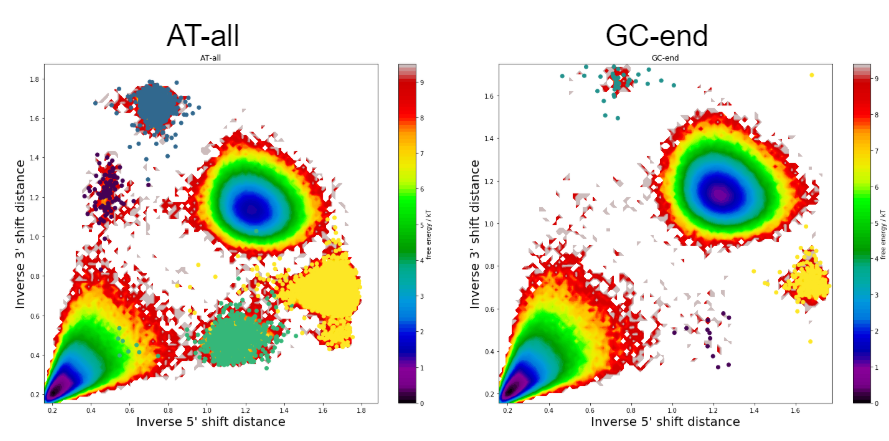
\includegraphics[width=\textwidth]{Figs/skeleton/shifting_distribution.PNG}
        \caption{Shows similarities between shifting modes and state memberships for AT-all and GC-ends (probs better to grey out underlying free energy landscape and move this to the SI.}
        \label{fig:shifting_distributions}
	\end{center}
\end{figure}

%%%%%%%%%%%%%%%%%%%%%%%%%%%%%%%%%%%%%%%%%%%%%%%%%%%%%%%%%%%%%%%%

\subsection{\label{sec:Results}GC-core}

The GC-core sequence represents a departure from the dominant slithering dynamics observed for AT-all and GC-end. Based on SRV cross-validation (SI), we select the first three components for our analysis. When correlating these first three modes with intermolecular distances (heatmap figure) we observe a similar first mode to the previous sequences reflecting the overall hybridization and dissociation process. The second mode no longer shows shifted diagonal behavior, but rather positive correlations between 5'/3' ends, negative correlations between 3'/3' and 5'/5' ends, and correlations closest to zero for the central GC pairs. Qualitatively, this suggests that the mode is picking up motions where base pair ends drift apart and opposite ends come closer together, while the oligo interior remains bound. The third mode shows symmetry along the main diagonal, much like the first mode but with an inverse trend. 

\begin{figure}[ht!]
	\begin{center}
        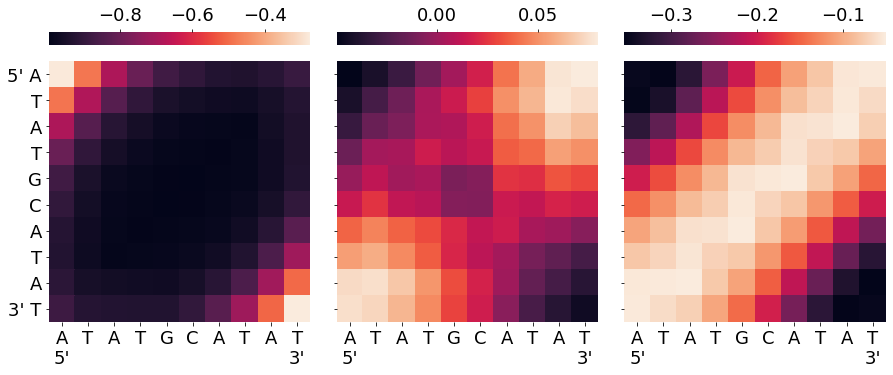
\includegraphics[width=\textwidth]{Figs/figs_0804/GC-core_srv_correlations.PNG}
        \caption{Shows Pearson correlations between leading SRV modes and all 100 intermolecular distances (needs labels for slow modes)}
        \label{fig:GC-core_srv_correlations}
	\end{center}
\end{figure}

(Not sure whether to include this section before or after building the MSM)
We examined each slow mode with respect to physical coordinates with which it showed high correlation. Unsurprisingly, the first mode tracks closely with the inverse distance between complement G:C pairs. These distances are the best indicators for a hybridization/dissociation, and we see a sharp change in the first SRV signal as these bonds form or break. The second slow mode is most active when the GC core pair are bound but the adjacent AT pairs are not. There is a small signal for fraying at the outer basepairs, but the mode overwhelmingly learns about these neighboring AT/GC bonds. This behavior reflects a kinetic trap between the core binding event and the fully hybridized (or evenly partially frayed) state. Previous work suggests that once key contacts are made, the zippering mechanism ensures that the helix will quickly form outward (cite). Our results indicate, however, that the relative instability of AT bonds compared the the GC-core can interrupt this process and form a longer lived frayed metastable states. This occurs during the dissociation process as well, where one half of the AT base contacts are entirely broken for a substantial period of time before the full dissociation event occurs. The third mode is most active during dissociation, and seems to track closely with the average distance between all complementary base pairs. We attribute this to the SRV learning about the slow diffusive motions of the two body system (not sure about this). In addition to picking up on dissociation behavior, the third mode seems to peak when the oligos are close together but configured in such a way that is not amenable hybridization. These misaligned conformations include inverse contacts where 5'/5' and 3'/3' ends meet, looped conformations where one strand is folded in on itself and preventing satisfactory WC contacts, or some combination of the two (SI third mode screenshots).

\begin{figure}[ht!]
	\begin{center}
        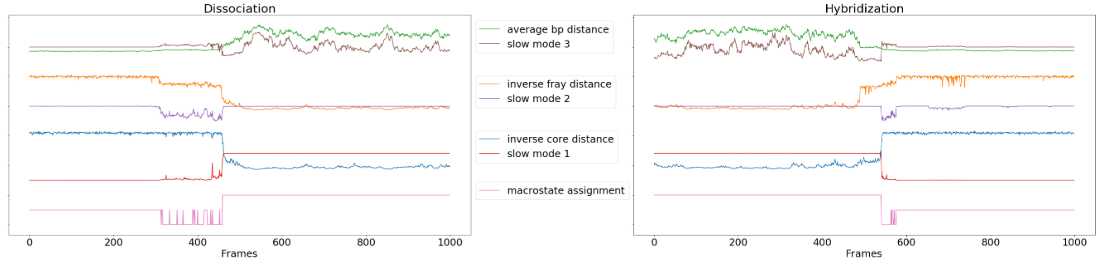
\includegraphics[width=\textwidth]{Figs/figs_0804/GC-core_tracking_modes.png}
        \caption{Show how SRV coordinates correspond to physical features over time and during sample dissociation and hybridization events.}
        \label{fig:GC-core_tracking_modes}
	\end{center}
\end{figure}

To further investigate these dynamics, we built an SRV-MSM using these first three SRV modes as a basis. We we found that four macrostate clustering was unstable -- likely because the 3rd mode is mostly providing  information about dissociation dynamics -- so we performed PCCA+ clustering into three macrostates representing the hybridized, dissociated, and "frayed" states. Again, we found transition probabilities between states and visualized representative molecular renderings. As we observed from the 2nd SRV mode analysis above, the "frayed" metatable state is solely composed of trajectories where both G:C core base pairs are bound and one of the adjacent A:T bonds are not. The MSM transition probabilities suggests that this is key intermediate state for both the hybridization and dissociation processes, however the pathways differ between directions. We find that the hybridized state has a 5x higher probability of transitioning into the frayed state within the lag time compared to transitions from the dissociated state. This make sense considering that this state is more accessible from an already bound helix. Moreover, once oligo are in this state, they are over 10x more likely to return to the hybridized state than to fully dissociate. Thus once a dissociated to frayed transition has occurred, it is a likely to proceed into a fully hybridized conformation. On the other hand, transitions from the hybridized to frayed state are much more frequent and are unlikely to proceed to a fully dissociated state.

\begin{figure}[ht!]
	\begin{center}
        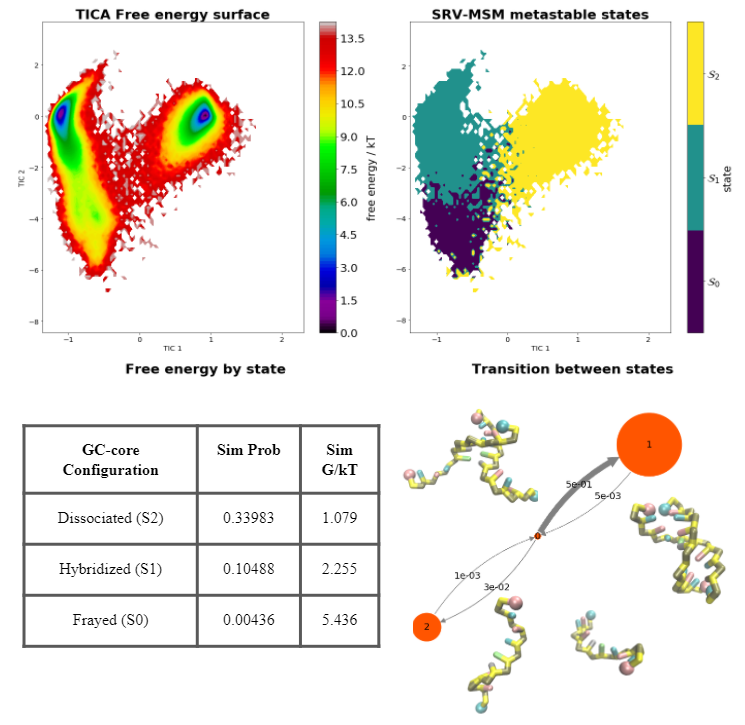
\includegraphics[width=\textwidth]{Figs/figs_0804/GC-core_thermo.PNG}
        \caption{Full MSM output for GC-core}
        \label{fig:GC-core_thermo}
	\end{center}
\end{figure}

When examining these same four sequences using T-jump and 2D spectroscopy, Sandstead et al. found that the GC-core had the highest deviation from two-state behavior during dissociation \citep{Sanstead2016}. As their analysis did not consider the previously mentioned shifted states, this intermediate state was defined by a high degree of fraying about the central core. While 1-2 base pair fraying was commonly observed for GC-mid and AT-all as well, lattice model predictions showed that GC-core had substantially more frayed base pairs. Further analysis showed that AT termini fraying was an effectively barrierless process characterized by rapid inter-conversion between all accessible frayed states \citep{Sanstead2018DirectDehybridization}. We see the same rapid fraying in simulation data (which too fast to be attributed with an SRV mode), however we stipulate that this inter-conversion first relies on the formation of the the AT-bond nearest to the GC center. In visualizing trajectories, we observe that the frayed ends rotate away from each other and impede helix formation, further highlighting the importance of this 4th base pair formation.


%%%%%% intro notes %%%%%%%
\citep{Sanstead2018DirectDehybridization} Good intro with many repesimportance of dynamics "rich dynamics even for short oligos"


Refs for DNA fraying:
\citep{Hagan2003AtomisticDNA} Atomistic simulations for biosensign app (can include in intro). Use TPS to focus on kinetic pathway by which singl base pair bind/unbind. Focus on end base of 3-bp oligomer in explicit solvent. Finds order parameters tracking base pair binding as well as intra-strand stacking. (energy and distance for each). 

\citep{Wong2008TheSimulations} Three step melting process: untwisting most important,

6K.-Y. Wong and B. M. Pettitt, “The pathway of oligomeric DNA melting investigated by molecular dynamics simulations,” Biophys. J. 95, 5618– 5626 (2008).
37A. Perez and M. Orozco, “Real-time atomistic description of DNA unfold- ing,” Angew. Chem. 49, 4805–4808 (2010).
38M. F. Hagan, A. R. Dinner, D. Chandler, and A. K. Chakraborty, “Atomistic understanding of kinetic pathways for single base-pair binding and unbinding

\subsection{\label{sec:Results}GC-mid}
\begin{enumerate}
	\item Evidence of fraying correlations in higher order modes, but these are not consistent and their inclusion does not generate a metastable third mode
	\item Treat this as a two-states model, where fraying is an expected feature of the hybridized state but not does not characterize a metastable state
	\item Show 2nd slow mode correlations in SI plus some configuration snapshots
	
\end{enumerate}  


%%%%%% Other MSM and timescales approaches  %%%%%%%%%%%
## Good references:

McGibbon, R. T., & Pande, V. S. (2015). Variational cross-validation of slow dynamical modes in molecular kinetics : Importance of not generating too many microstates and employting cross-validation to avoid artificially high scores or artificially slow dynamics. Both of these lead to models fitting statistical noise which is the root of boosted scores.

Pinamonti, G., Paul, F., Rodriguez, A., & Bussi, G. (n.d.). analyzed with core-set Markov state models, 43: Good ideas on core-based clustering. Assigning microstates based on physical characteristics is interesting but didn't seem to work for me in practice (could try doing this based on sim.log data with number of base pairs bound or some energy metric). Lot's of notes on this paper regarding comparisons to timescales. Good notes on higher resolution fraying interactions that we likely can't resolve.

Sua, E., Adelman, J. L., & Zuckerman, D. M. (2016). Accurate Estimation of Protein Folding and Unfolding Times : Beyond Markov State Models, 1. https://doi.org/10.1021/acs.jctc.6b00339:
More accurate ways to adapt MFPT into a rate


\begin{figure}[ht!]
	\begin{center}
        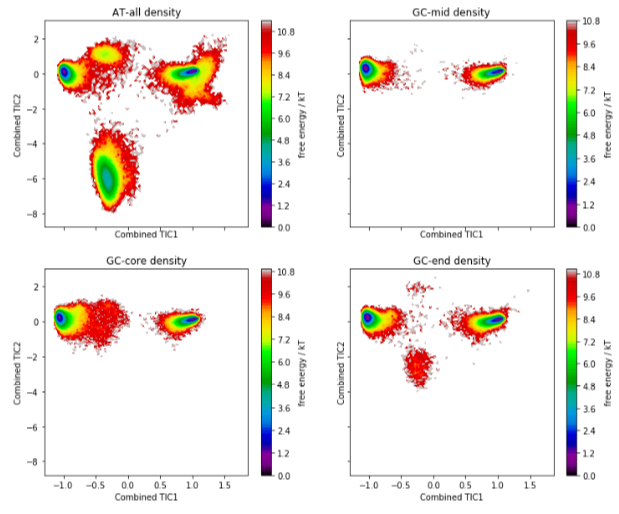
\includegraphics[width=\textwidth]{Figs/figs_0804/all_seq_tica_cvs.PNG}
        \caption{All sequences plotted on combined TICA axes}
        \label{fig:all_seq_tica_cvs}
	\end{center}
\end{figure}

\begin{figure}[ht!]
	\begin{center}
        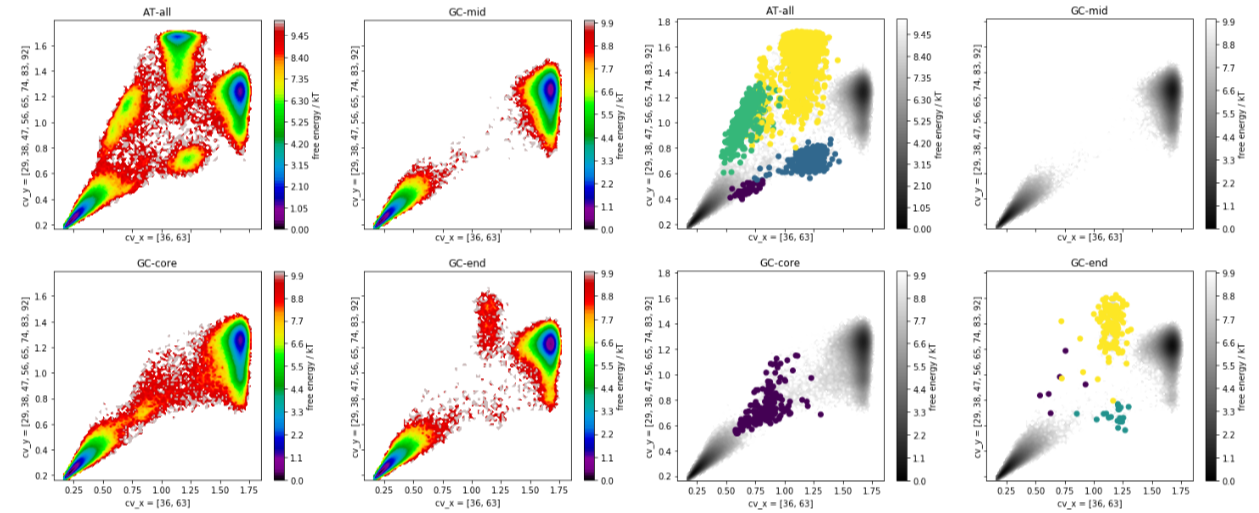
\includegraphics[width=\textwidth]{Figs/figs_0804/all_seq_physical_cvs.PNG}
        \caption{All sequences and metastable macrostates plotted on frayed/shifted collective variable axes}
        \label{fig:all_seq_physical_cvs}
	\end{center}
\end{figure}



\subsection{\label{sec:Results}Compare all results together}
\subsubsection{\label{sec:Results}Figure showing Pearson correlations between leading modes on common basis}


\subsubsection{\label{sec:Results}Figure showing all sequences plotted on a common low dimensional space (probably the 2nd TICA mode and the 2nd GC-core mode)}

\begin{enumerate}
	\item Evidence of fraying correlations in higher order modes, but these are not consistent and their inclusion does not generate a metastable third mode
	\item Treat this as a two-states model, where fraying is an expected feature of the hybridized state but not does not characterize a metastable state
\end{enumerate}

Nucleation-zipper mechnasism is a fast process that can orginate anywhere along the strand making it difficult to track..


\subsubsection{\label{sec:Results}Limitations} 
- not capturing zippering
One limititation of our appraoch that is that processes that are. For example, there are eight 3-bp sites on each oligo from which a zippering action coud nucleated. Because these are all unique sites (and zippering dynamics could vary at each site) it would be difficult to properly sample and interpret the unique corresponding mode. Furthermore these zippering dynamics occur significantly faster than slithering or GC-core fraying and cannot be captured via our save rate.


    
\section{\label{sec:conc}Conclusion}
\subsection{\label{sec:Results}Looks a lot like the abstract}



\clearpage
\newpage

%\bibliography{references}
Test cite: \citep{Zhang2018DeepMechanics}
\bibliography{refs_mendeley}

%%%%%%%%%%%%%%%%%%%%%%%%%%%%%%%%%%%%%%%%%%%%%%%%%%%%%%%%%%%%%%%%%%%%%
%% The "tocentry" environment can be used to create an entry for the
%% graphical table of contents.
%%%%%%%%%%%%%%%%%%%%%%%%%%%%%%%%%%%%%%%%%%%%%%%%%%%%%%%%%%%%%%%%%%%%%

\clearpage


\end{document}
